\subsection{Numerical simulation}
\label{subsec:ROSAA-simulation}

The ROSAA action spectroscopic technique, as described in Section \ref{subsec:ROSAA} utilises the change in attachment rate of rotation-specific energy levels to record the pure rotational spectrum. As depicted in Figure \ref{fig:setup:ROSAA} there are several competing processes involved in affecting the molecular ions population distribution on different rotational levels, and consequently affecting the obtained signal intensity. Therefore, in this section, we discuss a kinetic numerical model approach to understanding the ROSAA signal intensity.

\begin{figure}[!htb]
    \centering
    
    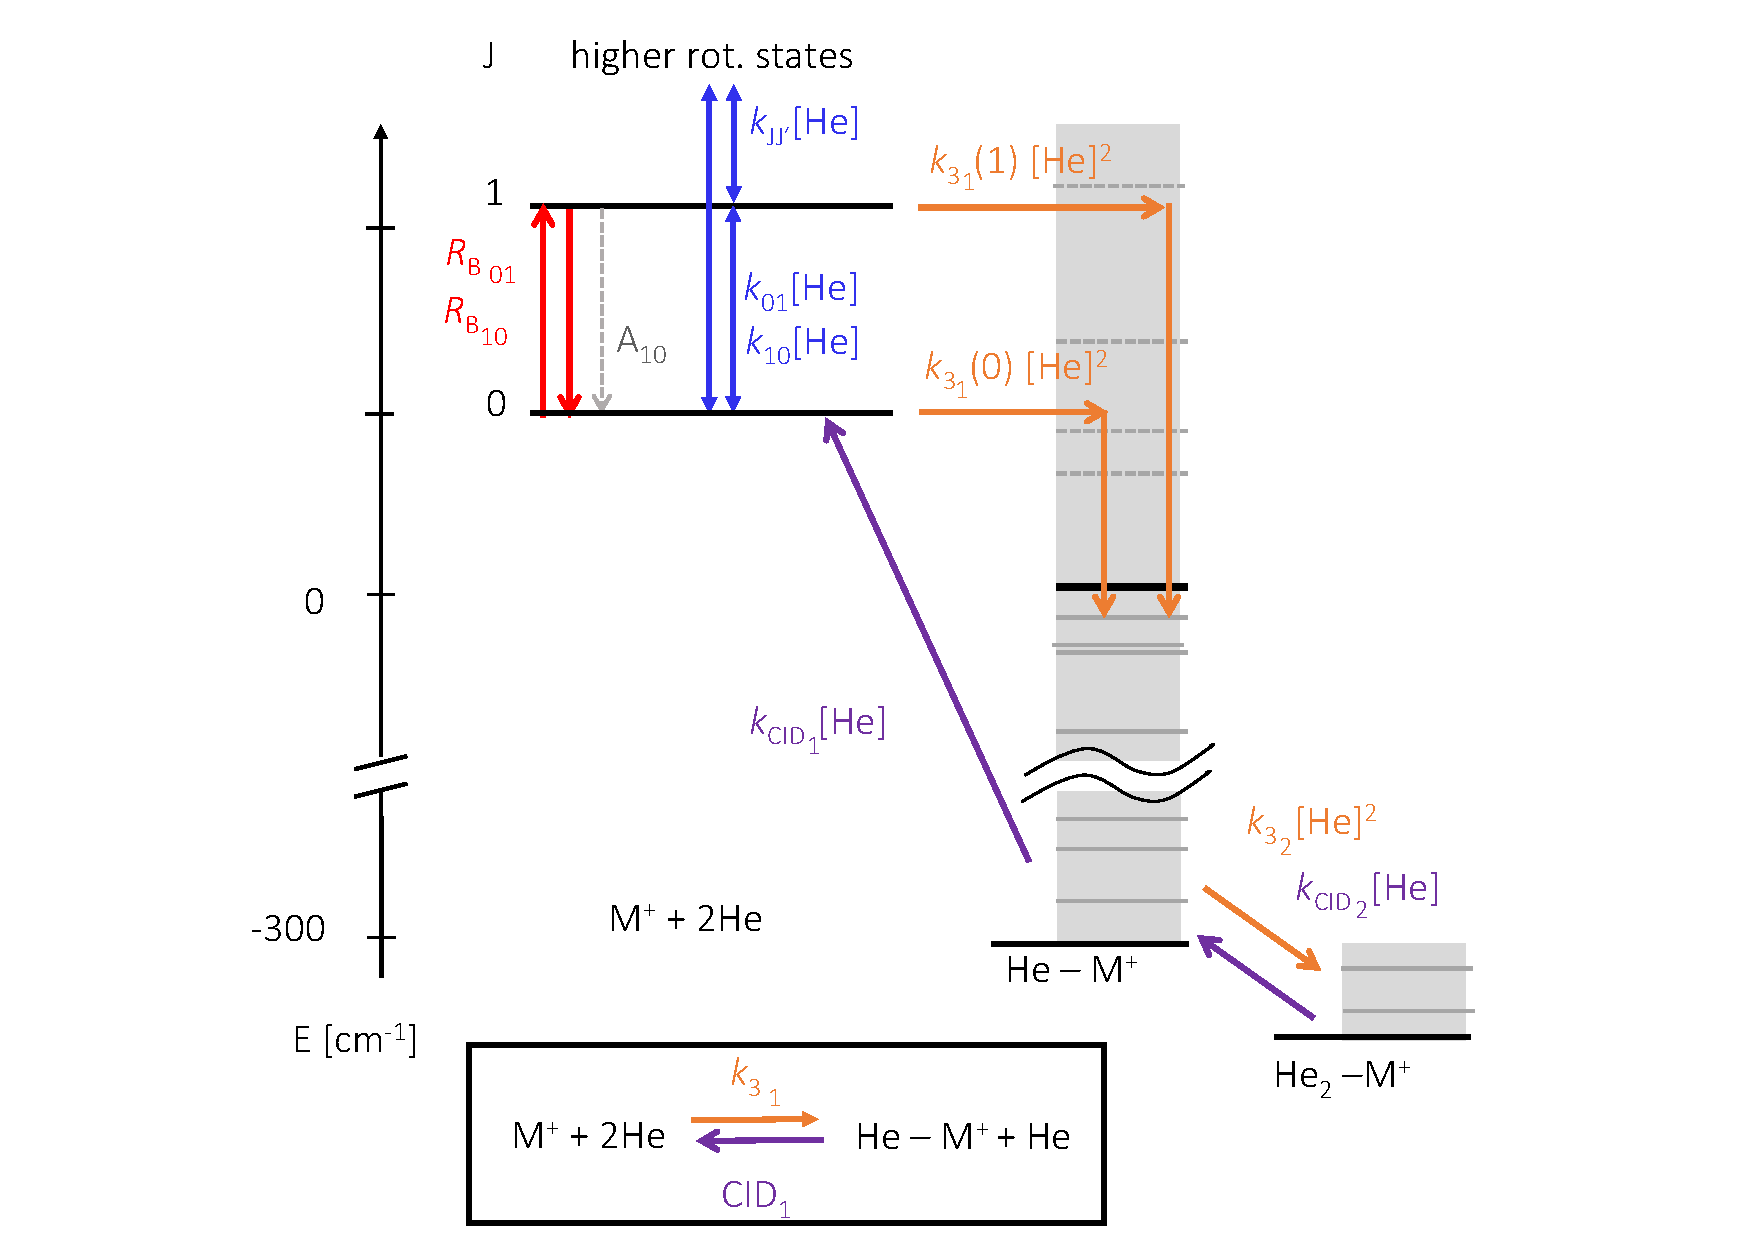
\includegraphics[width=1\textwidth]{figures/methods/ROSAA.pdf}
    \caption{Schematic kinetic model of the ROSAA action spectroscopic technique. The coloured labels and arrows indicate several competing processes for the reaction between the molecular ion M$^+$ and the neutral He atom. The typical rates for collisional (\textcolor{blue}{blue}) and radiative process (\textcolor{red}{red}) are in the range of $10^{4} - 10^{5}$ \pers, effective binary complex formation (\textcolor{orange}{orange}) is $> 0.01$ \pers\ and the collision-induced dissociation (\textcolor{violet}{violet}) is $> 0.1$ \pers\ at a given number density of $> 1 \cdot 10^{14}$ \percc. The spontaneous emission is labelled A$_{10}$, and rates are typically in order of $> 10^{-4}$ \pers. Figure adapted from \citet{Brunken2017}.}
    \label{fig:setup:ROSAA}
\end{figure}

% \textbf{Collisional process ($R_{if}$):}
% \subsubsection{Collisional process ($R$)}
\subsubsection{Collisional process (\texorpdfstring{$R$}\ )}
% \subsubsection{Collisional process (R)}
\label{subsec:ROSAA-simulation-coll}

As hot molecular ions (M$^+$) enter the trap (typical ambient trap temperature $\sim 4.5$ K) from the ion source (room temperature, 300 K or higher), they are collisionally cooled down by buffer gas atoms. The population distribution of rotational levels reaches a new equilibrium corresponding to the kinetic/collisional temperature ($T_{coll}$) of the system, which can be derived from the ion temperature ($T_{ion}$) as described in Section \ref{subsec:collisional-ion-temperature}. The rotational level-specific population ratio is given by:

\begin{equation}
    \left( \frac{dM^+_i}{dt} \right) _{coll.} = \sum_{f \neq i} R_{fi} \cdot M^+_f - R_{if} \cdot M^+_i
    \label{eqn:sim:coll}
\end{equation}
where $i$ and $f$ represents rotational states with rotational quantum numbers J= i, f, $if$ indicates initial $|i\rangle$ state transitions into final $|f\rangle$ state and $R_{if}$ corresponds to collisional rates [\pers] for $fi$ transition and given by 

\[ R_{if}=k_{if} \cdot [He] \]

where $k_{if}$ and $[He]$ indicate collisional rate coefficients and buffer gas (generally He gas) number density, respectively.\\

The rate coefficients can be derived from a quantum dynamical investigation using a closed coupling $M^+-$He rotational cross-section calculation method within a rigid body approach. However, in this study, no such investigations have been undertaken; the rate coefficient values ($k_{if}$) have been retrieved from the available literature. The fundamental detailed balancing relation is given as:

\begin{equation}
    \frac{k_{if}}{k_{fi}} = \frac{G_f}{G_i} e^{\Delta E / \left(k_B T \right)}
\end{equation}

where $g_i$ indicates statistical weight of corresponding $|i\rangle$ state ($G_J = 2J + 1$), $k_B$ is the Boltzmann constant, $T$ is the temperature of the system, and $\Delta E$ is the difference between final state energy ($\epsilon _f$) and initial state ($\epsilon _f$) energy, i.e.:
\[ \Delta E = \epsilon_f - \epsilon_i \]

At a given $T$ (actually $T_{coll}$), if only the collisional process is involved, solving equation \ref{eqn:sim:coll}, equilibrium values are reached typically in few $100 \sim\mu$s at $[He]\sim 10^{14}\ $\percc leading to a distribution equal to the Boltzmann population at $T$, i.e.:

\begin{equation}
    M^+_i = \frac
        {G_i \cdot e^{\epsilon_i / \left(k_B T \right)}}
        {\sum_{j=1}^{N} G_j \cdot e^{\epsilon_j / \left(k_B T \right)}}
        = \frac{{G_i \cdot e^{\epsilon_i / \left(k_B T \right)}}}{Z}
\end{equation}

where $N$ is the given system's total number of accessible rotational quantum levels, and $Z$ is the molecular partition function.\\ 

% \textbf{Spontaneous emission ($A_{fi}$):}
\subsubsection{Spontaneous emission (\texorpdfstring{$A$}\ )}
\label{subsec:ROSAA-simulation-spont}

It is the process in which a quantum mechanical system transits from an excited energy state to a lower lying energy state (e.g., its ground state) and emits a quantized amount of energy in the form of a photon. An initial state $|i\rangle$ with energy $\epsilon_i$ can decay to a final state $|f\rangle$ with energy $\epsilon_f$ via spontaneous emission of a photon with frequency ($\Delta \nu$). The Einstein A-coefficient gives the spontaneous emission rate [in photons per s]:

\[ A_{fi} = \frac{2\nu^3}{3\epsilon _0 h c^3} \cdot \mu _{fi}\]

where $\epsilon _0$, $h$, $c$ and $\mu _{fi}$ are vacuum permittivity, Planck's constant, speed of light and transition dipole moment, respectively. Including this emission process into Equation \ref{eqn:sim:coll} gives us the following relations:

\begin{equation}
    \left( \frac{dM^+_i}{dt} \right) _{coll. + Spont.} = \left( \frac{dM^+_i}{dt} \right) _{coll} + A_{fi}
    \label{eqn:sim:spontaneous-lower}
\end{equation}

\begin{equation}
    \left( \frac{dM^+_f}{dt} \right) _{coll. + Spont.} = \left( \frac{dM^+_i}{dt} \right) _{coll} - A_{fi}
    \label{eqn:sim:spontaneous-upper}
\end{equation}

The spontaneous rates are derived from the effective Hamiltonian fitting of a given molecular species using a program such as Pgopger \cite{western_pgopher_2017}. Typically, spontaneous emission rates are in the order of  $10^{-4}$ \pers which are smaller than collisional rates ($10^{3}-10^{5}$ \pers) at high number density ($>10^{14}$ \percc). Since the collisional processes dominate the spontaneous emission rates, for simplicity, the label $coll. + Spont.$ will just be referred as $coll.$.\\

\subsubsection{Radiative process (\texorpdfstring{$R_B$}{})}
\label{subsec:ROSAA-simulation-rad}

In the presence of radiation, the population is re-distributed again due to stimulated absorption ($B_{if}$) and emission ($B_{fi}$), described by the Einstein-B-coefficients. Both absorption and emission coefficients [m$^3$J$^{-1}$s$^{-2}$] can be derived from corresponding Einstein A-coefficient ($A_{fi}$):

\[ B_{fi} = \frac{c^3}{8\pi h \nu ^3} \cdot A_{fi} \]
\[ B_{if} = \frac{G_f}{G_i} \cdot B_{fi} \]

The rate of stimulated absorption, $R_{B_{if}}$ [in \pers], is given by:

\[ R_{B_{fi}} = B_{fi} \cdot \frac{P}{A_{trap} \cdot c} \cdot \text{V}(x;\sigma, \gamma) \]
where $A_{trap}=5 \cdot 10^{-5}$ m$^2$ indicates the area of 22-pole ion-trap, P corresponds to radiation power [in J$\cdot$ \pers], and $\text{V}(x;\sigma, \gamma)$ corresponds to Voigt profile lineshape (Eq. \ref{eqn:VoigtProfile}) for the rotation transition profile (x) with central frequency $\Delta \nu$.\\

Including the radiative process in Equation \ref{eqn:sim:spontaneous-lower} gives us the following rate equation:

\begin{equation}
    \left( \frac{dM^+_i}{dt} \right) _{coll. + Rad.} = \left( \frac{dM^+_i}{dt} \right) _{coll.}
     - R_{B_{if}} \cdot M^+_i + R_{B_{fi}} \cdot M^+_f
    \label{eqn:sim:radiative}
\end{equation}
\\

% \textbf{Attachment process ($R_3$ and $R_{CID}$):} 
\subsubsection{Attachment and dissociation process (\texorpdfstring{$R_3$ }{} and \texorpdfstring{$R_{CID}$}{} )}
\label{subsec:ROSAA-simulation-att}

The ternary association ($R_3$) and collision-induced dissociation ($R_{CID}$) rates [\pers] should also be included to complete the kinetic model scheme as shown in Figure \ref{fig:setup:ROSAA} (read Section \ref{subsec:rate-theory} for more detail on attachment process). The attachment process rates can be experimentally derived but only as a weighted average of all rotational population levels for a given molecular ion of interest (M$^+$). However, a rotational-specific rate is required for numerical simulation. The ratio of formation rate coefficients for the undergoing transitions is called $k_{3_1}$ ratio and will be referred to as \qt{$a$}:
\begin{equation}
    a = \frac{k_{3_1}(f)}{k_{3_1}(i)}
    \label{eqn:k3_ratio}
\end{equation}

The final master equation for numerical simulation of ROSAA technique involving $Coll. + Rad. + Att.$ for rotational transition from ground state $|i\rangle$ to excited state $|f\rangle$, and $M+ 2\text{He} $ attachment process is given by:

\begin{align*}
    \begin{split}
        \left( \frac{dM^+_{i}}{dt} \right) _{coll. + Att.+ Rad.} 
        & = \left( \frac{dM^+_{i}}{dt} \right) _{coll. +  Rad.}
    -R_{3_1} \cdot M^+_{i} + R_{CID_1} \cdot \text{He}M^+ \cdot p
    \\
    \left( \frac{dM^+_{f}}{dt} \right) _{coll. + Att.+ Rad.} 
    &= \left( \frac{dM^+_{f}}{dt} \right) _{coll. +Rad.}
    -R^{'}_{3_1} \cdot M^+_{f} + R_{CID_1} \cdot \text{He}M^+ \cdot (1-p)
    \end{split}
\end{align*}

where $R_{3_1}$ and $R^{'}_{3_1}$ correspond to state-dependent first-complex formation rates for ground and excited state, respectively. These rates can be expressed in terms of corresponding rate coefficients (\emph{k}) (read Section \ref{subsec:rate-theory} for more detail). \qt{\emph{p}} represents the collision-induced dissociation (CID) branching-ratio, \emph{i.e.,} the ratio of population transitions back to ground state from first complex (He$M^+$) via CID process.\\


The rate equations for the formation of the first two complex ions are given below (higher-order complexes can be treated accordingly):

\begin{equation*} \label{eq1}
    \begin{split}
        \frac{d\text{He}M^+}{dt} = 
            & +R_{3_1} \cdot M^+_i - R_{CID_1} \cdot \text{He}M^+ \cdot p \\
            &  +R^{'}_{3_1} \cdot M^+_f - R_{CID_1} \cdot \text{He}M^+ \cdot (1-p) \\
            & -R_{3_2} \cdot \text{He}M^+ + R_{CID_2} \cdot \text{He}_2M^+ \\
        \frac{d\text{He}_{2}M^+}{dt}
            &= +R_{3_2} \cdot \text{He}M^+ - R_{CID_2} \cdot \text{He}_{2}M^+
    \end{split}
\end{equation*}

% \textbf{Solving rate equations:} 
\subsubsection{Solving rate equations}
% \label{subsec:ROSAA-simulation-solution}

The processes involved in these numerical simulations are in widely varying timescales, as will be discussed in the corresponding chapters (see Chapter \ref{chapter:CD+} and \ref{chapter:CO+}). These rate equations are known as \enquote{stiff equations}. A stiff equation is a differential equation for which specific numerical methods  (explicit) for solving the equation are numerically unstable unless the step size is taken to be extremely small \cite{hairer_solving_1991}.  Therefore all of the ODEs discussed in this section are solved using the implicit Runge-Kutta method of the Radau IIA family of order 5 \cite{hairer_implementation_1996} using SciPy library \cite{virtanen_scipy_2020}.